\section{Equazioni di Lagrange e principi variazionali}
\subsection{Equazioni di Lagrange}
Talvolta le equazioni che seguono sono dette di Eulero--Lagrange, ma la derivazione che faremo è propriamente di Lagrange. Risale al 1788, con la pubblicazione del \emph{Mécanique Analytique}.

\note{Lezione 24/03/2026} L'equazione di Newton ha uso eminente nella dinamica del punto in un campo centrale e le equazioni cardinali nella dinamica del corpo rigido. Le equazioni di Lagrange sono invece utili per descrivere la dinamica dei sistemi con vincoli. Dimostreremo la corrispondenza biunivoca fra le equazioni di Newton, e quindi anche le equazioni cardinali, e le equazioni di Lagrange.

Consideriamo un sistema olonomo di punti materiali
\begin{equation*}
    \mathcal{S} = \{(\vP_1, m_1), \dots, (\vP_N, m_N)\},
\end{equation*}
di coordinate lagrangiane $q_1, \dots, q_n$.
Possiamo scrivere l'equazione di Newton per il sistema
\begin{equation*}
    m_i\,\vva_i = \vF_i + \vb{\Phi}_i \qquad i = 1, \dots, N,
\end{equation*}
dove $\vF_i$ è la risultante delle forze attive, le quali sono assegnate, per cui conosciamo una relazione
\begin{equation*}
    \vF_i = \vF_i(\vP_1, \dots, \vP_N; \vv_1, \dots, \vv_N; t);
\end{equation*}
e $\vb{\Phi}_i$ è la risultante delle forze vincolari, incognita.

D'Alembert riscrisse l'equazione come
\begin{equation}
    \label{eq:dalambert}
    (\vF_i -m_i\,\vva_i) + \vb{\Phi}_i = 0 \qquad i = 1, \dots, N,
\end{equation}
dove le forze del primo termine tra parentesi sono le \emph{forze perdute}, utilizzate per compensare le forze vincolari. Il principio di D'Alembert afferma che, per un sistema olonomo, le forze perdute e le forze vincolari si annullano reciprocamente.

Ci occuperemo di quello che viene detto \emph{problema fondamentale della dinamica dei sistemi olonomi}:
\begin{quote}
    Dato un sistema olonomo, le forze agenti su di esso e i vincoli, determinare il moto del sistema, note le condizioni iniziali (posizioni e velocità iniziali dei punti).
\end{quote}
Le incognite dinamiche del sistema sono le forze vincolari
\begin{equation*}
    \vb{\Phi}_1,\dots, \vb{\Phi}_N,
\end{equation*}
mentre le incognite cinematiche sono le accelerazioni e quindi le traiettorie dei punti
\begin{equation*}
    q_1(t), \dots, q_n(t).
\end{equation*}
Per cui in totale abbiamo $3N$ incognite dinamiche e $n$ incognite cinematiche, per un totale di $3N + n$ incognite.

Moltiplichiamo scalarmente l'equazione \eqref{eq:dalambert} per il vettore di spostamento virtuale $\var{\vP}_i$ e sommiamo su $i$ da $1$ a $N$:
\begin{equation*}
    \sum_{i=1}^N (\vF_i - m_i\,\vva_i + \vb{\Phi}_i)\cdot \var{\vP}_i = 0.
\end{equation*}
Abbiamo ridotto quindi $N$ equazioni vettoriali a una sola equazione scalare, al cui interno compaiono $\var{q}_1, \dots, \var{q}_n$ variazioni indipendenti.
Distribuendo il prodotto scalare, otteniamo
\begin{equation*}
    \underbrace{\sum_{i=1}^N \vF_i\cdot \var{\vP}_i}_{\var{L^{(a)}}}  \underbrace{-\sum_{i=1}^N m_i\,\vva_i\cdot \var{\vP}_i}_{\var{L^{(m)}}} + \underbrace{\sum_{i=1}^N \vb{\Phi}_i\cdot \var{\vP}_i}_{\var{L^{(v)}}} = 0,
\end{equation*}
ovvero la somma di tre lavori, dove $m_i\,\vva_i$ è dimensionalmente una forza, detta \emph{forza di inerzia}. Otteniamo così il \emph{principio di D'Alembert} propriamente detto
\begin{equation*}
    \var{L^{(a)}} + \var{L^{(m)}} + \var{L^{(v)}} = 0.
\end{equation*}

Consideriamo l'ipotesi di vincoli ideali, per cui $\var{L^{(v)}} \geq 0$. \note{Le equazioni di Lagrange possono essere ricavate allo stesso modo introducendo i moltiplicatori di Lagrange} Segue necessariamente 
\begin{equation*}
    \var{L^{(a)}} + \var{L^{(m)}} \leq 0.
\end{equation*}
Consideriamo l'ulteriore ipotesi di vincoli bilaterali ideali, per cui $\var{L^{(v)}} = 0$. Segue di conseguenza
\begin{equation*}
    \var{L^{(a)}} + \var{L^{(m)}} = 0.
\end{equation*}

Possiamo esplicitare le incognite $q_1, \dots, q_n$ attraverso le componenti lagrangiane delle forze attive nel calcolo del lavoro virtuale
\begin{equation*}
    \var{L^{(a)}} = \sum_{i=1}^N \vF_i\cdot \var{\vP}_i = \sum_{j=1}^n Q_j\,\var{q}_j,
\end{equation*} dove
\begin{equation*}
    Q_j = \sum_{i=1}^N \vF_i\cdot \pdv{\vP_i}{q_j}.
\end{equation*}
Introduciamo analogamente le componenti lagrangiane delle forze di inerzia
\begin{equation*}
    \var{L^{(m)}} = \sum_{h=1}^N -m_h\,\vva_h\cdot \var{\vP}_h = \sum_{k=1}^n \tau_k\,\var{q}_k,
\end{equation*}
dove \begin{equation*}
    \tau_k = \sum_{i=1}^N -m_i\,\vva_i\cdot \pdv{\vP_i}{q_k}.
\end{equation*}
Il principio di D'Alembert si riscrive quindi come
\begin{equation*}
    \tau_h + Q_h = 0 \qquad h = 1, \dots, n,
\end{equation*}
ovvero $n$ equazioni scalari finite\note{non compaiono più variazioni infinitesime}. Queste sono le \emph{equazioni di Lagrange}, tuttavia non sono ancora poste in una formulazione comoda.

\begin{lemma}[Legge di cancellazione dei punti]
    In un sistema olonomo vale la seguente relazione
    \begin{equation*}
        \pdv{\vv}{\dot{q}_h} = \pdv{\vP}{q_h},
    \end{equation*}
    dove
    \begin{equation*}
        \vv = \dot{\vP}.
    \end{equation*}
\end{lemma}
\begin{proof}
    Abbiamo che
    \begin{equation*}
        \vv = \dv{\vP}{t} = \sum_{k=1}^n \pdv{\vP}{q_k}\,\dot{q}_k + \pdv{\vP}{t}.
    \end{equation*}
    Derivando rispetto a $\dot{q}_h$ otteniamo
    \begin{equation*}
        \pdv{\vv}{\dot{q}_h} = \sum_{k=1}^n \pdv{\vP}{q_k}\,\delta_{kh} = \pdv{\vP}{q_h}.
    \end{equation*}
\end{proof}

Applicando questa legge alla componente lagrangiana della forza di inerzia, otteniamo
\begin{align*}
    \tau_h &= \sum_{i=1}^N -m_i\,\vva_i\cdot \pdv{\vP_i}{q_h} \\ 
    &= -\sum_{i=1}^N m_i\,\dv{\vv_i}{t}\cdot \pdv{\vP_i}{q_h} \\
    &= -\dv{t}\sum_{i=1}^N m_i\,\vv_i\cdot \pdv{\vP_i}{q_h} + \sum_{i=1}^N m_i\,\vv_i\cdot \dv{t}\pdv{\vP_i}{q_h} \\
    &= -\dv{t}\sum_{i=1}^N m_i\,\vv_i\cdot \pdv{\vv}{\dot{q}_h} + \sum_{i=1}^N m_i\,\vv_i\cdot \pdv{\vv}{q_h} \note{Legge di cancellazione dei punti e Teorema di Schwartz}\\
    &= -\dv{t}\pdv{\dot{q}_h}\sum_{i=1}^N \frac{1}{2}m_i\,\vv_i^2 + \pdv{q_h}\sum_{i=1}^N \frac{1}{2}m_i\,\vv_i^2 \\
    &= -\dv{t}\pdv{T}{\dot{q}_h} + \pdv{T}{q_h},
\end{align*}
questi ultimi termini vengono detti \emph{binomi di Lagrange}.

Otteniamo quindi le \emph{equazioni di Lagrange nella seconda forma}
\begin{equation*}
    \dv{t}\pdv{T}{\dot{q}_h} - \pdv{T}{q_h} = Q_h \qquad h = 1, \dots, n,
\end{equation*}
con le $2n$ condizioni iniziali
\begin{equation*}
    \begin{cases}
        q_1(t_0)= q_1^0, \dots, q_n(t_0) = q_n^0, \\
        \dot{q}_1(t_0) = \dot{q}_1^0, \dots, \dot{q}_n(t_0) = \dot{q}_n^0.
    \end{cases}
\end{equation*}
Le equazioni di Lagrange sono $n$ equazioni differenziali ordinarie del secondo ordine pure (ovvero dove non compaiono le reazioni vincolari) nelle incognite $q_1(t), \dots, q_n(t)$.\note{Compaiono le derivate parziali dell'energia cinetica, che però non è un'incognita} Il numero di equazioni è precisamente uguale al numero di gradi di libertà del sistema, ottenendo quindi una notevole semplificazione rispetto alle $3N$ equazioni di Newton.

Non è immediato assumere che valga il teorema di esistenza e unicità per le equazioni di Lagrange. Sicuramente sono verificate le ipotesi di continuità e lipschitzianità. Il teorema prevede un'equazione differenziale in forma normale, ovvero
\begin{equation*}
    y' = f(x, y),
\end{equation*}
con la derivata di ordine massimo espressa in funzione delle altre variabili.

Possiamo espandere la seguente derivata
\begin{equation*}
    \dv{t}\pdv{T}{\dot{q}_h} = \sum_{k=1}^n \pdv[2]{T}{\dot{q}_h}{\dot{q}_k}\,\ddot{q}_k + \sum_{k=1}^n \pdv[2]{T}{\dot{q}_h}{q_k}\,\dot{q}_k + \pdv[2]{T}{\dot{q}_h}{t}.
\end{equation*}
È possibile isolare il termine del secondo ordine e portarlo al primo membro, ottenendo
\begin{equation*}
    \sum_{k=1}^n \pdv[2]{T}{\dot{q}_h}{\dot{q}_k}\,\ddot{q}_k = \underbrace{Q_h + \pdv{T}{q_h} - \sum_{k=1}^n \pdv[2]{T}{\dot{q}_h}{q_k}\,\dot{q}_k - \pdv[2]{T}{\dot{q}_h}{t}}_{F_h(\vq, \dot{\vq}, t)}.
\end{equation*}
Inoltre, si verifica velocemente che il termine $\pdv[2]{T}{\dot{q}_h}{\dot{q}_k}$ è il termine $h, k$ della matrice di massa $(a_{hk})$, ottenendo quindi
\begin{equation*}
    \sum_{k=1}^n a_{hk}\,\ddot{q}_k = F_h(\vq, \dot{\vq}, t).
\end{equation*}
Pertanto,
\begin{align*}
    A \ddot{\vq} &= \vF(\vq, \dot{\vq}, t) \\
    \implies \ddot{\vq} &  = A^{-1} \vF(\vq, \dot{\vq}, t)
\end{align*}
e quindi
\begin{equation*}
    \ddot{q}_h= G_h(\vq, \dot{\vq}, t) \qquad h = 1, \dots, n,
\end{equation*}
avendo quindi scritto l'equazione in forma normale. Il teorema di esistenza e unicità è quindi verificato.

\note{Lezione 31/03/2026} L'unicità delle soluzioni garantisce il \emph{determinismo}, idea fondamentale nel '700 per cui una volta che sono note le condizioni iniziali, è possibile stabilire univocamente il comportamento del sistema nel tempo. A livello sperimentale questa idea non regge a causa della presenza di errori sulle misure.

Consideriamo ora un sistema di forze attive indipendenti dalle velocità, quindi con componenti lagrangiane del tipo
\begin{equation*}
    Q_h = Q_h(\vq, t) \qquad h = 1, \dots, n,
\end{equation*}
e supponiamo che esiste una funzione $V(\vq, t)$, almeno di classe $C^1$, tale che
\begin{equation*}
    Q_h = -\pdv{V}{q_h} \iff \var{L^{(a)}} = -\var{V}.
\end{equation*}
Queste forze non sono necessariamente conservative, ma sono comunque derivate da un potenziale.

In questo caso, le equazioni di Lagrange si riscrivono come
\begin{equation*}
    \dv{t}\pdv{T}{\dot{q}_h} - \pdv{T}{q_h} = -\pdv{V}{q_h},
\end{equation*}
ovvero
\begin{equation*} 
    \dv{t} \pdv{(T-V)}{\dot{q}_h} - \pdv{(T-V)}{q_h} = 0.\note{dove $\pdv{V}{\dot{q}_h} = 0$}
\end{equation*}
Introducendo la funzione
\begin{equation*}
    L \defeq T - V,
\end{equation*}
detta \emph{lagrangiana} del sistema, possiamo scrivere le equazioni di Lagrange nella loro forma più nota, dette di Eulero--Lagrange:
\begin{equation*}
    \dv{t}\pdv{L}{\dot{q}_h} - \pdv{L}{q_h} = 0
\end{equation*}

\begin{definition}[Potenziale generalizzato]
    Diremo che un sistema di forze con componenti $Q_h = Q_h(\vq, \dot{\vq}, t)$,
    dipende da un \emph{potenziale generalizzato} $V = V(\vq, \dot{\vq}, t)$ se
    \begin{equation*}
        Q_h = \dv{t}\pdv{V}{\dot{q}_h}-\pdv{V}{q_h}.
    \end{equation*}
\end{definition}

In questo caso, le equazioni di Lagrange si riscrivono come
\begin{equation*}
 \dv{t}\pdv{T}{\dot{q}_h} - \pdv{T}{q_h} = \dv{t}\pdv{V}{\dot{q}_h}-\pdv{V}{q_h},
\end{equation*}
ovvero, utilizzando la lagrangiana,
\begin{equation*}
    \dv{t}\pdv{L}{\dot{q}_h} - \pdv{L}{q_h} = 0.
\end{equation*}

\begin{example}[Forze derivate da un potenziale generalizzato]
    Le seguenti forze derivano da un potenziale generalizzato
    \begin{itemize}
        \item Forza di Coriolis nei sistemi non inerziali;
        \item Forza di Lorentz in elettromagnetismo.
    \end{itemize}
\end{example}

\begin{example}[Applicazione delle equazioni di Lagrange ad un sistema rigido]
    Consideriamo un'asta rigida omogenea, di massa $m$ e lunghezza $\ell$, i cui estremi sono costretti a scorrere in assenza di attrito lungo due assi ortogonali. Si precisa che gli assi costituiscono guide puramente cinematiche e non corpi fisici materiali; il moto dell'asta non è quindi ostacolato dalla loro intersezione.
    
    \begin{figure}[ht]
    \centering
    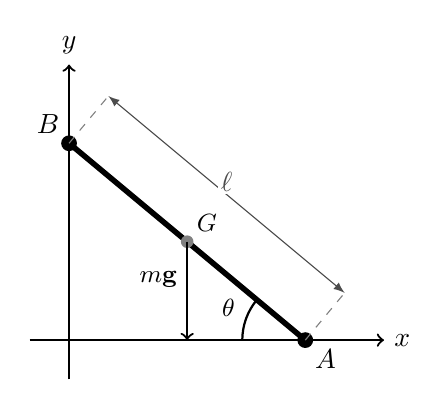
\begin{tikzpicture}
        % Axes (extended slightly into the negative for better visual balance)
        \draw[thick, ->] (-0.5, 0) -- (4, 0) node[right] {$x$};
        \draw[thick, ->] (0, -0.5) -- (0, 3.5) node[above] {$y$};
        
        % Rod without text node (label \ell will be on the bracket)
        \draw[line width=2pt, black] (3, 0) -- (0, 2.5);
        
        % End points
        \fill[black] (3, 0) circle (0.1) node[below right] {$A$};
        \fill[black] (0, 2.5) circle (0.1) node[above left] {$B$};
        
        % Center of mass (G)
        \fill[gray] (1.5, 1.25) circle (0.08);
        % Position G label better: above and slightly to the right of the G point
        \node[above right, font=\small] at (1.5, 1.25) {$G$};
        
        % Length bracket \ell - offset from the rod for clarity
        % Leader 1 from A(3,0) outwards perpendicular to the rod
        \draw[dashed, black!50] (3,0) -- (3.5, 0.6);
        % Leader 2 from B(0,2.5) outwards perpendicular to the rod
        \draw[dashed, black!50] (0,2.5) -- (0.5, 3.1);
        % Dimension line with double arrows and label \ell
        \draw[<->, >=latex, black!70] (3.5, 0.6) -- (0.5, 3.1) node[midway, above, fill=white, inner sep=1pt] {$\ell$};

        % Angle arc \theta, centered at A(3,0). Shows angle with horizontal.
        \draw[thick] (3,0) + (180:0.8) arc (180:140.2:0.8);
        \node[font=\small, yshift=-5.5pt, xshift=-5pt] at (2.2, 0.6) {$\theta$};

        % Force: Weight (P) applied at G, thick vector
        \draw[thick, black, ->] (1.5, 1.25) -- (1.5, 0.0);
        \node[left, font=\small, yshift=5pt] at (1.5, 0.6) {$m\mathbf{g}$}; % Weight label clean-up

    \end{tikzpicture}
    \caption{Asta rigida con estremi scorrevoli sugli assi.}
    \end{figure}

    Il sistema ha un grado di libertà, per cui possiamo scegliere come coordinata generalizzata l'angolo $\theta$ che l'asta forma con l'asse $x$.

    Calcoliamo l'energia potenziale attraverso il lavoro virtuale. I vincoli del sistema sono bilaterali e fissi, quindi il lavoro virtuale corrisponde a quello reale. Essendo la forza peso rivolta verso il basso lungo l'asse $y$, si ha:
    \begin{equation*}
        \var{L} = \vF\cdot \var{\vG} = -mg\var{y_G},
    \end{equation*}
    dove $y_G$ è la coordinata $y$ del centro di massa dell'asta. Dalla geometria del sistema ricaviamo:
    \begin{equation*}
        \begin{cases}
            x_G = \frac{\ell}{2}\cos\theta \\
            y_G = \frac{\ell}{2}\sin\theta \\    
        \end{cases}
        \implies \var{y_G} = \frac{\ell}{2}\cos\theta\,\var{\theta}.
    \end{equation*}
    Otteniamo quindi:
    \begin{align*}
        \var{L} &= -mg\frac{\ell}{2}\cos\theta\,\var{\theta} = -\var{V} \\
        \implies \var{V} &= mg\frac{\ell}{2}\cos\theta\,\var{\theta} \\
        \implies V(\theta) &= mg\frac{\ell}{2}\sin\theta.
    \end{align*}
    Troviamo ora l'energia cinetica del sistema. Utilizziamo il teorema di König:
    \begin{equation*}
        T= \frac{1}{2}m\,v_G^2 + \frac{1}{2}I_G\,\dot{\theta}^2,
    \end{equation*}
    dove $I_G$ è il momento di inerzia dell'asta rispetto al centro di massa.
    Calcoliamo $v_G^2$ derivando le coordinate:
    \begin{equation*}
        v_G^2 = \dot{x}_G^2 + \dot{y}_G^2 = \left(-\frac{\ell}{2}\sin\theta\,\dot{\theta}\right)^2 + \left(\frac{\ell}{2}\cos\theta\,\dot{\theta}\right)^2 = \frac{\ell^2}{4}\dot{\theta}^2.
    \end{equation*}
    Il momento di inerzia è dato da:
    \begin{equation*}
        I_G =  \int_{-\frac{\ell}{2}}^{\frac{\ell}{2}} \rho \,\xi^2 \dd{\xi} = \frac{m}{\ell} \left[\frac{\xi^3}{3}\right]_{-\frac{\ell}{2}}^{\frac{\ell}{2}} = \frac{1}{12}m\ell^2.
    \end{equation*}
    Combinando i due risultati, otteniamo:
    \begin{equation*}
        T = \frac{1}{2}m\frac{\ell^2}{4}\dot{\theta}^2 + \frac{1}{2}\left(\frac{1}{12}m\ell^2\right)\dot{\theta}^2 = \frac{1}{6}m\ell^2\dot{\theta}^2.
    \end{equation*}

    La lagrangiana del sistema $L = T - V$ è quindi:
    \begin{equation*}
        L = \frac{1}{6}m\ell^2\dot{\theta}^2 - mg\frac{\ell}{2}\sin\theta.
    \end{equation*}
    Scriviamo quindi le equazioni di Lagrange:
    \begin{gather*}
        \dv{t}\pdv{L}{\dot{\theta}} - \pdv{L}{\theta} = 0 \\
        \implies \frac{1}{3}m\ell^2\ddot{\theta} + \frac{1}{2}mg\ell\cos\theta = 0.
    \end{gather*}
    Come dalla teoria possiamo scrivere l'equazione in forma normale
    \begin{equation*}
        \ddot{\theta} = -\frac{3}{2}\frac{g}{\ell}\cos\theta.
    \end{equation*}
\end{example}


\subsection{Trasformazioni di coordinate}
Stabilita una trasformazione di coordinate nello spazio delle configurazioni
\begin{equation*}
    \xi_i = \xi_i(\vq, t) \qquad i = 1, \dots, n,
\end{equation*}
che sia localmente invertibile, ovvero
\begin{equation*}
    \det\left(\pdv{\xi_i}{q_j}\right) \neq 0,
\end{equation*}
vogliamo stabilire che forma prendono le equazioni di Lagrange nelle nuove coordinate $\xi_i$. Definendo la nuova lagrangiana
\begin{equation*}
    L^* = [L(\vq, \dot{\vq}, t)]_{\vq = \vq(\vb{\xi})},
\end{equation*}
possiamo scrivere le equazioni di Lagrange nella nuova coordinata $\xi_i$ come
\begin{equation*}
    \dv{t}\pdv{L^*}{\dot{\xi}_i} - \pdv{L^*}{\xi_i} = 0 \qquad i = 1, \dots, n.
\end{equation*}

\subsection{Leggi di conservazione e teorema di Noether}
\note{Lezione 07/04/2026}

Consideriamo un sistema di lagrangiana $L(\vq, \dot{\vq}, t)$ e un moto del sistema fissando $\vq(t)$ e $\dot{\vq}(t)$. Calcoliamo la derivata totale di $L$ rispetto al tempo:
\begin{equation*}
    \dv{L}{t} = \sum_{h=1}^n \pdv{L}{q_h}\,\dot{q}_h + \underbrace{\sum_{h=1}^n \pdv{L}{\dot{q}_h}\,\ddot{q}_h}_{*} + \pdv{L}{t}.
\end{equation*}
Attraverso la regola di derivazione del prodotto, otteniamo
\begin{align*}
    \dv{L}{t} &= \sum_{h=1}^n \pdv{L}{q_h}\,\dot{q}_h + \dv{t}\sum_{h=1}^n \pdv{L}{\dot{q}_h}\,\dot{q}_h - \sum_{h=1}^n \dv{t}\pdv{L}{\dot{q}_h}\,\dot{q}_h + \pdv{L}{t} \\
    &= \dv{t} \sum_{h=1}^n \pdv{L}{\dot{q}_h}\,\dot{q}_h + \sum_{h=1}^n \left(\pdv{L}{q_h} - \dv{t}\pdv{L}{\dot{q}_h}\right)\dot{q}_h + \pdv{L}{t} \\
\end{align*}
Il secondo termine è nullo in virtù delle equazioni di Lagrange. Otteniamo quindi
\begin{equation*}
    \dv{L}{t} = \dv{t} \sum_{h=1}^n \pdv{L}{\dot{q}_h}\,\dot{q}_h + \pdv{L}{t}.
\end{equation*}
Riordinando i termini, otteniamo
\begin{equation}
    \label{eq:conservazione_H}
    \dv{t}\left(\sum_{h=1}^n \pdv{L}{\dot{q}_h}\,\dot{q}_h - L\right) = -\pdv{L}{t}.
\end{equation}

\begin{definition}[Funzione di Jacobi]
    Definiamo \emph{funzione di Jacobi} di un sistema la funzione
    \begin{equation*}
        h(\vq, \dot{\vq}, t) = \sum_{h=1}^n \pdv{L}{\dot{q}_h}\,\dot{q}_h - L.
    \end{equation*}
\end{definition}

Dall'equazione \eqref{eq:conservazione_H} segue il seguente teorema di conservazione.

\begin{theorem}
    Sia $\mathcal{S}$ un sistema di lagrangiana $L$. Se $\pdv{L}{t} = 0$, allora la funzione di Jacobi $h$ è una costante del moto; cioè:
    \begin{equation*}
        \dv{h}{t} = 0 \iff h = \text{costante}.
    \end{equation*}
\end{theorem}

\begin{definition}[Momenti generalizzati]
    I momenti generalizzati di un sistema sono le quantità
    \begin{equation*}
        p_i = \pdv{L}{\dot{q}_i} \qquad i = 1, \dots, n.
    \end{equation*}
\end{definition}
Questi momenti sono immediate generalizzazioni della quantità di moto Newtoniana
\begin{equation*}
    \vp = m\vv,
\end{equation*}

\subsubsection{Conservazione dell'energia}
Consideriamo ora un sistema meccanico olonomo soggetto a forze attive di potenziale $V(\vq)$, per cui la lagrangiana è, attraverso l'equazione \eqref{eq:energia_cinetica},
\begin{equation*}
    L = T - V = T_0 + T_1 + T_2- V.
\end{equation*}
Sviluppando la funzione di Jacobi, otteniamo
\begin{align*}
    h &= \sum_{h=1}^n \pdv{L}{\dot{q}_h}\,\dot{q}_h - L \\
    &= \sum_{h=1}^n \left(\pdv{T_1}{\dot{q}_h} + \pdv{T_2}{\dot{q}_h}\right)\dot{q}_h - T_0 - T_1 - T_2 + V.
\end{align*}

Ricorriamo al teorema di Eulero sulle funzioni omogenee:
\begin{theorem}[di Eulero sulle funzioni omogenee]
    Sia $f(\vx)$ una funzione omogenea di grado $\alpha$ in $\R^n$, ovvero
    \begin{equation*}        
        f(\lambda \vx) = \lambda^\alpha f(\vx) \qquad \forall \lambda > 0.
    \end{equation*}
    Allora
    \begin{equation*}
        \sum_{i=1}^n x_i\,\pdv{f}{x_i} = \alpha f.
    \end{equation*}
\end{theorem}

Otteniamo quindi
\begin{align*}
    h &= 2T_2 +  T_1 - T_1 - T_2 - T_0 + V \\
    &= T_2 - T_0 + V.
\end{align*}
Se il sistema è a vincoli fissi e soggetto a forze attive conservative risulta
\begin{equation*}
    h = T_2 + V = T + V  = E,
\end{equation*}
dove $E$ è l'energia meccanica totale.

Per cui, quando il sistema è conservativo, la funzione di Jacobi coincide con l'energia meccanica totale, che quindi si conserva. Tuttavia, la funzione di Jacobi si conserva anche in sistemi non conservativi, fornendo una generalizzazione della legge di conservazione dell'energia, motivo per cui talvolta la funzione di Jacobi è detta \emph{energia generalizzata}.

\subsubsection{Generalizzazione delle leggi di conservazione}
\begin{definition}[Integrale primo]
    Sia un sistema di lagrangiana $L$. Diremo che una funzione $f(\vq, \dot{\vq}, t)$ è un \emph{integrale primo} delle equazioni di Lagrange se $f$ si conserva costante lungo le soluzioni di tali equazioni.
\end{definition}

In altri termini, presa una soluzione $\vq(t)$ delle equazioni di Lagrange, se $f$ è un integrale primo, si ha
\begin{equation*}
    \dv{f(\vq(t), \dot{\vq}(t), t)}{t} = 0 \quad \forall t \iff f(\vq(t), \dot{\vq}(t), t) = \text{costante} \quad \forall t.
\end{equation*}

\begin{definition}[Coordinata ciclica]
    Sia un sistema di lagrangiana $L$. Diremo che una coordinata $q_i$ è una \emph{coordinata ciclica} o \emph{ignorabile} se la lagrangiana non dipende esplicitamente da $q_i$, ovvero
    \begin{equation*}
        \pdv{L}{q_i} = 0.
    \end{equation*}
\end{definition}

\begin{remark}
    Se $q_i$ è una coordinata ciclica, allora il momento $p_i$ generalizzato (o coniugato) a $q_i$ si conserva costante. Questo risultato discende direttamente dalle equazioni di Lagrange, che in questo caso si riducono a
    \begin{equation*}
        \dv{t}\pdv{L}{\dot{q}_i} = \pdv{L}{q_i} = 0 \implies \pdv{L}{\dot{q}_i} = p_i = \text{costante}.
    \end{equation*}
\end{remark}

\begin{definition}[Trasformazione di coordinate ammissibile]
    Sia un sistema di lagrangiana $L$. Diremo che una trasformazione di coordinate $Q_i = f_i(\vq)$ indipendente dal tempo è \emph{ammissibile} per $L$ se
    \begin{equation*}
        L(\vQ, \dot{\vQ}) = L(\vq, \dot{\vq}).
    \end{equation*}
\end{definition}

\begin{definition}[Gruppo di trasformazioni ammissibili]
    Diremo che una famiglia ad un parametro $\vf(\vq, s)$, con $s \in \R$, di trasformazioni ammissibili costituisce un gruppo di trasformazioni ammissibili per $L$ se
    \begin{enumerate}[label=($\roman*$)]
        \item $\vf(\vq, 0) = \vq \quad \forall \vq$;
        \item $\vQ = f(\vq, s) \implies \vq = \vf(\vQ, -s) \quad \forall s$.
        \item $\vf(\vf(\vq, s_1), s_2) = \vf(\vq, s_1 + s_2) \quad \forall s_1, s_2$.
    \end{enumerate}
\end{definition}

\begin{theorem}[di Noether]
    \note{del 1918}
    Sia $\vf(\vq, s)$ un gruppo di trasformazioni ammissibili per la lagrangiana $L$ di un sistema. Allora, la funzione
    \begin{equation*}
        I(\vq, \dot{\vq}) = \sum_{j=1}^n \pdv{L}{\dot{q}_j}\,\pdv{f_j}{s}\bigg|_{s=0}
    \end{equation*}
    è una costante del moto.
\end{theorem}
\begin{proof}
    Osserviamo che
    \begin{equation*}
        L(\vf(\vq, s), \dot{\vf}(\vq, s)) = L(\vq, \dot{\vq}) \quad \forall s.
    \end{equation*}
    Derivando rispetto $s$ otteniamo
    \begin{align*}
        0 = \dv{s} L\left(\vf(\vq, s), \dot{\vf}(\vq, s)\right) &= \sum_{j=1}^n \pdv{L}{q_j}\,\pdv{f_j}{s} + \sum_{j=1}^n \pdv{L}{\dot{q}_j}\,\pdv{\dot{f_j}}{s} \\
        &= \sum_{j=1}^n \pdv{L}{q_j}\,\pdv{f_j}{s} + \dv{t}\sum_{j=1}^n \pdv{L}{\dot{q}_j}\,\pdv{f_j}{s} - \sum_{j=1}^n \dv{t}\pdv{L}{\dot{q}_j}\,\pdv{f_j}{s} \\
        &=  \sum_{j=1}^n \left(\pdv{L}{q_j} - \dv{t}\pdv{L}{\dot{q}_j}\right)\pdv{f_j}{s} + \dv{t}\sum_{j=1}^n \pdv{L}{\dot{q}_j}\,\pdv{f_j}{s}.
    \end{align*}

    Posto $s = 0$, otteniamo
    \begin{equation*}
        0 = \sum_{j=1}^n \left(\pdv{L}{q_j} - \dv{t}\pdv{L}{\dot{q}_j}\right)\pdv{f_j}{s}\bigg|_{s=0} + \dv{t}\sum_{j=1}^n \pdv{L}{\dot{q}_j}\,\pdv{f_j}{s}\bigg|_{s=0}.
    \end{equation*}
    Il primo termine è nullo in virtù delle equazioni di Lagrange e l'assioma $(i)$ del gruppo, per cui
    \begin{equation*}
        \dv{t}\sum_{j=1}^n \pdv{L}{\dot{q}_j}\,\pdv{f_j}{s}\bigg|_{s=0} = 0,
    \end{equation*}
    ovvero
    \begin{equation*}
        I = \sum_{j=1}^n \pdv{L}{\dot{q}_j}\,\pdv{f_j}{s}\bigg|_{s=0} = \text{costante}.
    \end{equation*}
\end{proof}

\note{Lezione 13/04/2026}
\begin{example}
    Consideriamo la seguente famiglia di trasformazioni
    \begin{equation*}
        f_j(\vq,s) = \begin{cases}
        q_i + s,\quad &j=i\\
        q_j, \quad &j\neq i
        \end{cases}.
    \end{equation*}
    Abbiamo
    \begin{equation*}
        \pdv{f_j}{s}\bigg|_{s=0} = \begin{cases}
        1, \quad &j=i\\
        0, \quad &j\neq i
        \end{cases}
    \end{equation*}
    e quindi
    \begin{equation*}
        I(\vq, \dot{\vq}) = \sum_{j=1}^n \pdv{L}{\dot{q}_j}\,\pdv{f_j}{s}\bigg|_{s=0} = \pdv{L}{\dot{q}_i} = p_i.
    \end{equation*}

    Per cui se il sistema è invariante per traslazioni lungo la coordinata $q_i$, allora essa è ciclica e il momento generalizzato $p_i$ si conserva costante.
\end{example}

\subsection{Formulazione variazionale}
Passiamo ora a una formulazione alternativa della dinamica, basata su principi \emph{variazionali}. L'idea guida è descrivere il moto attraverso un problema di estremo relativo per una quantità integrale.

Un esempio storico fondamentale è il \emph{problema della brachistocrona}, formulato da Johann Bernoulli nel 1696:\note{Il nome "brachistocrona" deriva dal greco "brachistos" (più breve) e "chronos" (tempo), indicando la curva che consente il percorso più rapido tra due punti sotto l'effetto della gravità.}
\begin{quote}
    In un piano verticale si considerino due punti $A$ e $B$, non sulla stessa verticale, con $A$ più alto di $B$. Supponiamo, inoltre, di collegare $A$ e $B$ con una guida curva liscia $\gamma$.
    
    Qual è la curva $\gamma$ che minimizza il tempo di percorrenza di una particella che, lasciata cadere da $A$ con velocità iniziale nulla, scende lungo la guida fino a raggiungere $B$?
\end{quote}
    \begin{figure}[ht]
        \centering
        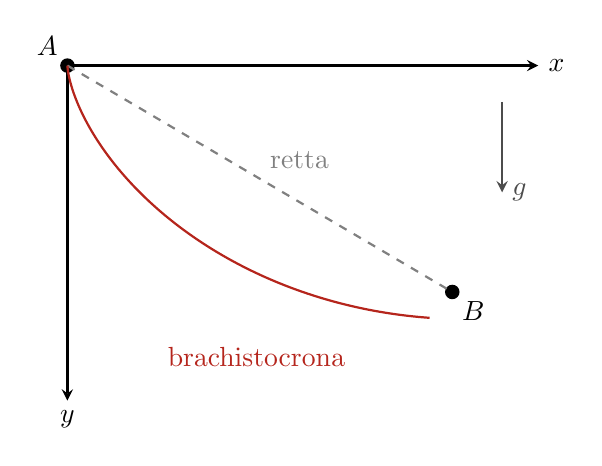
\begin{tikzpicture}[>=stealth, scale=1.15]
            % Sistema di assi con origine in A e asse y rivolto verso il basso.
            \draw[thick, ->] (0, 0) -- (5.2, 0) node[right] {$x$};
            \draw[thick, ->] (0, 0) -- (0, -3.7) node[below] {$y$};

            % Punti iniziale e finale
            \fill[black] (0, 0) circle (0.08) node[above left] {$A$};
            \fill[black] (4.25, -2.5) circle (0.08) node[below right] {$B$};

            % Riferimento: percorso rettilineo
            \draw[dashed, gray, thick] (0, 0) -- (4.25, -2.5) node[midway, above right] {retta};

            % Brachistocrona (arco di cicloide)
            \draw[thick, BrickRed] plot[domain=0:3.0, samples=150, variable=\t]
                ({1.4*(\t - sin(\t r))}, {-1.4*(1 - cos(\t r))});
            \node[BrickRed, below right] at (1, -3) {brachistocrona};

            % Direzione della gravita'
            \draw[thick, ->, black!70] (4.8, -0.4) -- (4.8, -1.4) node[right] {$\vb{g}$};
        \end{tikzpicture}
        \caption{Problema della brachistocrona: confronto tra il percorso rettilineo e la curva cicloidale che minimizza il tempo di discesa da $A$ a $B$.}
        \label{fig:brachistocrona}
    \end{figure}

La prima traiettoria che viene in mente è una linea retta, perché minimizza la distanza geometrica. Tuttavia, tenendo conto della gravità, può risultare più conveniente un percorso inizialmente più ripido: la particella acquista velocità prima e il tempo totale di percorrenza si riduce. La soluzione del problema è un arco di cicloide.

Questo problema viene considerato il punto di inizio del calcolo delle variazioni, nonostante la presenza di problemi simili in epoca precedente, come il \emph{problema della Regina Didone}.

Per formulare il problema in modo analitico, consideriamo l'integrale primo dell'energia per il sistema della brachistocrona.
\begin{equation*}
    \frac{1}{2}mv^2 - mg y = \frac{1}{2}mv_0^2 + mg y_0 = 0,
\end{equation*}
otteniamo quindi
\begin{equation*}
    \frac{1}{2}\dv{s}{t}^2 - g y = 0 \implies \dv{s}{t} = \sqrt{2 g y}.
\end{equation*}
Separando le variabili, otteniamo
\begin{equation*}
    \dd{t} = \frac{\dd{s}}{\sqrt{2 g y}},
\end{equation*}
e quindi, integrando 
\begin{equation*}
    T = \int_0^T \dd{t} = \int_0^{x_1} \frac{\dd{s}}{\sqrt{2 g y}} = \frac{1}{\sqrt{2g}}\int_0^{x_1} \sqrt{\frac{1+y'^2}{y}}\dd{x}.
\end{equation*}

Poiché il fattore $\frac{1}{\sqrt{2g}}$ è una costante positiva, minimizzare $T$ equivale a minimizzare il funzionale
\begin{equation*}
    \tau = \int_0^{x_1} \sqrt{\frac{1+y'^2}{y}}\dd{x}.
\end{equation*}

La tecnica appena usata si generalizza a una classe ampia di problemi.

\begin{definition}[Funzionali integrali del calcolo delle variazioni]
    Un \emph{funzionale integrale} è una funzione che associa ad ogni funzione $y(x)$, definita su un intervallo $[x_0, x_1]$, un numero reale attraverso un'integrazione del tipo
    \begin{equation*}
        I[y] = \int_{x_0}^{x_1} F(y, y', x)\dd{x},
    \end{equation*}
    dove $y\in C^0([x_0, x_1])\cap C^1(x_0, x_1)$.

    La funzione $F\in C^2([x_0, x_1] \times \mathbb{R} \times \mathbb{R})$ è detta \emph{lagrangiana} per analogia con il caso meccanico.
\end{definition}

L'insieme di tutte le funzioni $y(x)$ definite su $[x_0, x_1]$ e appartenenti a $C^0([x_0, x_1])\cap C^1(x_0, x_1)$ ha un ruolo analogo al domionino di una funzione reale e viene detto \emph{classe di funzioni ammissibili}.

Consideriamo il caso di un massimo relativo del funzionale. Per analogia con il caso di una funzione reale di una variabile, diremo che $I[y]$ è massimo in $y^*(x)$ se, per ogni funzione $y(x)$ sufficientemente vicina a $y^*(x)$, si ha
\begin{equation*}
    I[y] \leq I[y^*].
\end{equation*}

Definiamo la \emph{variazione} infinitesima \note{o perturbazione} di $y^*(x)$ come
\begin{align*}
    y(x) = y^*(x) + \alpha \eta(x), \quad &\forall \alpha \in (-\varepsilon, \varepsilon), \\
    &\forall \eta \in C^0([x_0, x_1])\cap C^1(x_0, x_1): \eta(x_0) = \eta(x_1) = 0.
\end{align*}

\begin{figure}[h!]
    \centering
    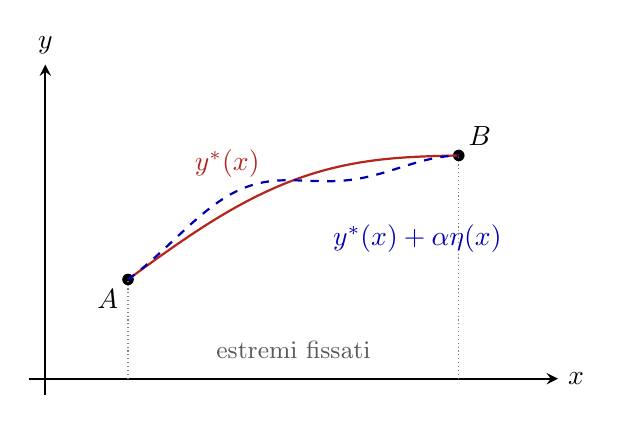
\begin{tikzpicture}[>=stealth, scale=1.05]
        % Assi
        \draw[thick, ->] (-0.2, 0) -- (6.2, 0) node[right] {$x$};
        \draw[thick, ->] (0, -0.2) -- (0, 3.8) node[above] {$y$};

        % Estremi fissati
        \coordinate (A) at (1, 1.2);
        \coordinate (B) at (5, 2.7);
        \fill[black] (A) circle (0.07) node[below left] {$A$};
        \fill[black] (B) circle (0.07) node[above right] {$B$};

        % Funzione di riferimento y*
        \draw[thick, BrickRed, smooth] plot[domain=1:5, samples=120, variable=\x]
            (\x, {1.2 + 1.5*((\x-1)/4) + 0.45*sin(180*(\x-1)/4)});
        \node[BrickRed] at (2.2, 2.6) {$y^*(x)$};

        % Variazione y* + alpha eta con stessi estremi
        \draw[thick, blue!70!black, dashed, smooth] plot[domain=1:5, samples=120, variable=\x]
            (\x, {1.2 + 1.5*((\x-1)/4) + 0.45*sin(180*(\x-1)/4) + 0.25*sin(180*(\x-1)/4)*sin(360*(\x-1)/4)});
        \node[blue!70!black] at (4.5, 1.7) {$y^*(x)+\alpha\eta(x)$};

        % Indicatori di estremi fissi
        \draw[densely dotted, gray] (1, 0) -- (1, 1.2);
        \draw[densely dotted, gray] (5, 0) -- (5, 2.7);
        \node[font=\small, gray!70!black] at (3, 0.35) {estremi fissati};
    \end{tikzpicture}
    \caption{Esempio di funzione di riferimento $y^*(x)$ e di una variazione ammissibile $y^*(x)+\alpha\eta(x)$: le curve coincidono agli estremi perché $\eta(x_0)=\eta(x_1)=0$.}
    \label{fig:variazioni_estremi_fissi}
\end{figure}

La condizione $\eta(x_0)=\eta(x_1)=0$ è essenziale: significa che le perturbazioni ammissibili non modificano i valori agli estremi, cioè i punti iniziale e finale restano fissati. In questo modo stiamo confrontando curve che soddisfano gli stessi vincoli al bordo; la ricerca dell'estremo relativo avviene quindi solo tra funzioni con i medesimi estremi.

\begin{definition}[Estremi relativi di un funzionale]
        Diremo che $y^*(x)$ è un massimo relativo per il funzionale $I[y]$ se
        \begin{align*}
            I[y^*] \geq I[y^* + \alpha \eta], \quad
            &\forall \alpha \in (-\varepsilon, \varepsilon), \\
            &\forall \eta \in C^0([x_0, x_1])\cap C^1(x_0, x_1): \eta(x_0) = \eta(x_1) = 0.
        \end{align*}
        Analogamente, diremo che $y^*(x)$ è un minimo relativo se
        \begin{align*}
            I[y^*] \leq I[y^* + \alpha \eta], \quad 
            &\forall \alpha \in (-\varepsilon, \varepsilon), \\
            &\forall \eta \in C^0([x_0, x_1])\cap C^1(x_0, x_1): \eta(x_0) = \eta(x_1) = 0.
        \end{align*}
\end{definition}

Introduciamo il \emph{lemma fondamentale del calcolo delle variazioni}, che risulta utile per dimostrare il teorema di Eulero che lo segue.

\begin{lemma}[fondamentale del calcolo delle variazioni]
    Sia $\eta \in C^0([a, b])\cap C^1(a, b)$ con $\eta(a) = \eta(b) = 0$. Se
    \begin{equation*}
        \int_{a}^{b} G(x)\,\eta(x)\dd{x} = 0 \quad \forall \eta,
    \end{equation*}
    allora $G(x) = 0$ per ogni $x\in [a, b]$.
\end{lemma}
\begin{proof}
    Supponiamo per assurdo che esista $\xi\in (a,b): G(\xi) \neq 0$. Senza perdita di generalità, supponiamo che $G(\xi) > 0$. Per il teorema della permanenza del segno, esiste un intervallo $[\xi_1, \xi_2] \subset (a, b)$, tale che $G(x) > 0\ \forall x\in [\xi_1, \xi_2]$.

    Poniamo
    \begin{equation*}
        \eta(x) = \begin{cases}
            0, \quad &x\in [a, \xi_1)\cup (\xi_2, b] \\
            (x-\xi_1)^2(\xi_2-x)^2, \quad &x\in [\xi_1, \xi_2]\note{moltiplicando la potenza per $n$ è possibile dimostrare il lemma anche con funzioni $C^n$}
        \end{cases}.
    \end{equation*}
    Ovviamente abbiamo che $\eta\in C^0([a, b])\cap C^1(a, b)$ e $\eta(a) = \eta(b) = 0$. Tuttavia, con questa scelta di $\eta$ otteniamo
    \begin{equation*}
        \int_{a}^{b} G(x)\,\eta(x)\dd{x} = \int_{\xi_1}^{\xi_2} G(x)\,(x-\xi_1)^2(\xi_2-x)^2\dd{x} > 0,
    \end{equation*}
    in contraddizione con l'ipotesi. Pertanto possiamo concludere che $G(x) = 0$ per ogni $x\in [a, b]$.
\end{proof}

\begin{theorem}[di Eulero] \note{analogo del teorema di Fermat per le funzioni reali}
    Sia un funzionale integrale
    \begin{equation*}
        I[y] = \int_{x_0}^{x_1} F(y, y', x)\dd{x}.
    \end{equation*}
    Una condizione necessaria affinché $y^*(x)$ sia un estremo relativo di $I[y]$ è che essa soddisfi l'equazione
    \begin{equation*}
        \pdv{F}{y} - \dv{x}\pdv{F}{y'} = 0,
    \end{equation*}
    detta equazione di Eulero--Lagrange del funzionale $I[y]$.
\end{theorem}
\begin{proof}
    Supponiamo che $y^*(x)$ sia un massimo relativo per $I$, ovvero
    \begin{align*}
        I[y^*] \geq I[y^* + \alpha \eta], \quad
        &\forall \alpha \in (-\varepsilon, \varepsilon), \\
        &\forall \eta \in C^0([x_0, x_1])\cap C^1(x_0, x_1): \eta(x_0) = \eta(x_1) = 0.
    \end{align*}
    Osserviamo che la mappa 
    \begin{equation*}
        \alpha \mapsto I[y^* + \alpha \eta] = \int_{x_0}^{x_1} F(y^* + \alpha \eta, y^{*'} + \alpha \eta', x)\dd{x}
    \end{equation*}
    è una funzione reale di una variabile reale, derivabile rispetto ad $\alpha$. Inoltre ha un massimo in $\alpha = 0$, quindi la sua derivata prima in $\alpha = 0$ è nulla. Calcoliamo allora
    \begin{align*}
        \dv{I}{\alpha} &= \dv{\alpha} \int_{x_0}^{x_1} F(y^* + \alpha \eta, y^{*'} + \alpha \eta', x)\dd{x} \\ 
        &= \int_{x_0}^{x_1} \left(\pdv{F}{y}\,\eta + \pdv{F}{y'}\,\eta'\right)\dd{x} \\
        &= \int_{x_0}^{x_1}\left\{ \pdv{F}{y}\eta + \dv{x}\left(\pdv{F}{y'}\eta\right) - \dv{x}\pdv{F}{y'}\eta \right\} \dd{x} \\
        &= \int_{x_0}^{x_1} \left(\pdv{F}{y} - \dv{x}\pdv{F}{y'}\right)\eta\dd{x} + \int_{x_0}^{x_1} \dv{x}\left(\pdv{F}{y'}\eta\right) \dd{x}\\
        &= \int_{x_0}^{x_1} \left(\pdv{F}{y} - \dv{x}\pdv{F}{y'}\right)\eta\dd{x} + \left[\pdv{F}{y'}\eta\right]_{x_0}^{x_1}
    \end{align*}
    Il secondo termine è nullo in virtù della condizione $\eta(x_0) = \eta(x_1) = 0$, per cui
    \begin{equation*}
        \dv{I}{\alpha}\bigg|_{\alpha=0} = \int_{x_0}^{x_1} \left(\pdv{F}{y} - \dv{x}\pdv{F}{y'}\right)\eta\dd{x} = 0 \quad \forall \eta.
    \end{equation*}
    Applicando il lemma fondamentale del calcolo delle variazioni, otteniamo
    \begin{equation*}
        \pdv{F}{y} - \dv{x}\pdv{F}{y'} = 0,
    \end{equation*}
    ovvero $y^*(x)$ soddisfa l'equazione di Eulero--Lagrange del funzionale $I[y]$.
\end{proof}

Introduciamo la seguente notazione per indicare una variazione infinitesima di $y$:
\begin{equation*}
    \var{y} = \alpha \eta.
\end{equation*}
Notiamo che vale la seguente relazione
\begin{equation*}
    (\var{y})' = \alpha \eta' = \var{y'}.
\end{equation*}

\begin{definition}[Operatore variazionale di Lagrange]
    Dato un funzionale $I[y]$, definiamo la \emph{variazione prima di $I$} come
    \begin{equation*}
        \var{I} \defeq \left(\dv{I}{\alpha}\right)_{\alpha=0}.
    \end{equation*}
\end{definition}
Sviluppando i conti, otteniamo il seguente sviluppo:
\begin{align*}
    I[y^* + \var{y}] &= I[y^*] + \alpha \int_{x_0}^{x_1} \left[\pdv{F}{y}\eta + \pdv{F}{y'}\eta'\right] \dd{x} + \dots
\end{align*}
Integrando per parti il secondo termine e applicando le condizioni al contorno, ricaviamo la variazione prima:
\begin{equation*}
    \var{I} = \int_{x_0}^{x_1} \left[\pdv{F}{y} - \dv{x} \pdv{F}{y'}\right] \alpha \eta \dd{x} = \int_{x_0}^{x_1} \left[\pdv{F}{y} - \dv{x} \pdv{F}{y'}\right] \var{y} \dd{x}.
\end{equation*}
Possiamo quindi riscrivere lo sviluppo finale di $I[y^* + \var{y}]$ in modo rigoroso unendo i due risultati:
\begin{equation*}
    I[y^* + \var{y}] = I[y^*] + \int_{x_0}^{x_1} \left[\pdv{F}{y} - \dv{x} \pdv{F}{y'}\right] \var{y} \dd{x} + \dots
\end{equation*}

Considerando, invece, una n-upla di funzioni, definiamo un funzionale integrale del tipo
\begin{equation*}
    I[y_1, \dots, y_n] = I[\vb{y}]= \int_{x_0}^{x_1} F(\vb{y}, \vb{y'}, x)\dd{x}.
\end{equation*}
il teorema di Eulero si generalizza in maniera immediata, fornendo un sistema di $n$ equazioni differenziali alle derivate ordinarie:
\begin{theorem}[di Eulero per più variabili]
    Sia un funzionale integrale
    \begin{equation*}        I[\vb{y}, \vb{y'}] = \int_{x_0}^{x_1} F(\vb{y}, \vb{y'}, x)\dd{x}.
    \end{equation*}
    Una condizione necessaria affinché $\vb{y}^*(x)$ sia un estremo relativo di $I[\vb{y}, \vb{y'}]$ è che essa soddisfi il sistema di equazioni
    \begin{equation*}
        \pdv{F}{y_i} - \dv{x}\pdv{F}{y_i'} = 0 \qquad i = 1, \dots, n.
    \end{equation*}
\end{theorem}
La dimostrazione è del tutto analoga a quella del teorema di Eulero per una sola variabile, con la differenza che si deve considerare una variazione infinitesima di ogni funzione $y_i$, ottenendo alla fine
\begin{equation*}
    0 = \left(\dv{I}{\alpha}\right)_{\alpha=0} = \int_{x_0}^{x_1} \sum_{i=1}^n \left[\pdv{F}{y_i} - \dv{x}\pdv{F}{y_i'}\right] \eta_i \dd{x} \quad \forall \eta_1, \dots, \eta_n,
\end{equation*}
e quindi
\begin{equation*}
    \pdv{F}{y_i} - \dv{x}\pdv{F}{y_i'} = 0 \qquad i = 1, \dots, n.
\end{equation*}

\begin{definition}[Funzionale stazionario]
    Sia un funzionale integrale
    \begin{equation*}
        I[y] = \int_{x_0}^{x_1} F(y, y', x)\dd{x}.
    \end{equation*}
    Diremo che $y^*(x)$ rende \emph{stazionario} il funzionale $I[y]$ se $y^*(x)$ soddisfa l'equazione di Eulero--Lagrange del funzionale $I[y]$ e equivalentemente
    \begin{equation*}
        \var{I} = 0.
    \end{equation*}
\end{definition}

\subsection{Principio di Hamilton}
La grande applicazione del calcolo variazionale alla meccanica analitica è il \emph{principio di Hamilton} o \emph{principio di azione stazionaria}. Il principio per secoli è stato detto della \emph{minima} azione, a causa di un'errata convinzione che l'azione fosse sempre minimizzata.

\begin{theorem}[Principio di Hamilton]\note{(1834)}
    Sia $\mathcal{S}$ un sistema olonomo di coordinate $\vq$ e lagrangiana $L$, e siano $P_0$ e $P_1$ due configurazioni assunte da $\mathcal{S}$ agli istanti $t_0$ e $t_1$, rispettivamente. Tra le possibili traiettorie che collegano $P_0$ a $P_1$\note{$P_0$ e $P_1$ sono punti dello spazio delle configurazioni} in un intervallo di tempo $[t_0, t_1]$, il modo effettivo del sistema è quello in corrispondenza della traiettoria che rende stazionario il funzionale
    \begin{equation*}
        A = \int_{t_0}^{t_1} L(\vq, \dot{\vq}, t) \dd{t},\note{Solitamente si indica con $S$}
    \end{equation*}
    detto \emph{azione} del sistema. Ovvero
    \begin{equation*}
        \var{A} = 0.
    \end{equation*}
\end{theorem}
È importante sottolineare che il principio di Hamilton non dipende dalla scelte delle coordinate, ma solo dalla lagrangiana, che è una funzione scalare. \note{Lezione 21/04/2026} Inoltre, tale formulazione permette di riconoscere i moti \emph{globalmente}, rispetto alla formulazione locale delle equazioni di Lagrange.

Introdotto il principio di Hamilton, è possibile dimostrare la seguente proprietà delle equazioni di Lagrange:
\begin{proposition}
    Le equazioni di Lagrange sono invarianti per trasformazioni puntuali di coordinate.
\end{proposition}
\begin{proof}
    Sia $L$ la lagrangiana di un sistema in coordinate $\vq$ e sia $\vQ = \vf(\vq)$ una trasformazione puntuale di coordinate. La lagrangiana del sistema in coordinate $Q_i$ è data da
    \begin{equation*}
        L^*(\vQ, \dot{\vQ}, t) = L(\vq, \dot{\vq}, t).
    \end{equation*}
    Poiché $L$ e $L^*$ sono la stessa funzione scalare si ha
    \begin{equation*}
        \int_{t_1}^{t_2} L^*(\vQ, \dot{\vQ}, t) \dd{t} = \int_{t_1}^{t_2} L(\vq, \dot{\vq}, t) \dd{t} \implies \var{A^*} = \var{A},
    \end{equation*}
    dove abbiamo
    \begin{equation*}
        \vq(\vQ, t), \quad \dot{\vq}(\vQ, \dot{\vQ}, t).
    \end{equation*}
    Pertanto, se $A$ è stazionario, allora anche $A^*$ è stazionario, e viceversa. Di conseguenza, le equazioni di Lagrange in coordinate $\vq$ e in coordinate $\vQ$ sono equivalenti, ovvero
    \begin{equation*}
        \pdv{L}{q_i} - \dv{t}\pdv{L}{\dot{q}_i} = 0 \iff \pdv{L^*}{Q_i} - \dv{t}\pdv{L^*}{\dot{Q}_i} = 0.
    \end{equation*}
\end{proof}
